\chapter{\MakeUppercase{Постановка задачи и план решения}}

\section{Задачи работы}

В рамках работы рассматривается разработка шагающего четырехногого робота, с упором на проблему проектирования конечностей и разработки программного обеспечения для управления движением.

Для выполнения работы требуется:
\begin{itemize}
    \item Разработать общую кинематическую схему робота.
    \item Рассчитать худший (по нагрузке) статический случай для конечностей 4-х ногого робота.
    \item Подобрать электроприводы удовлетворяющие по крутящему моменту.
    \item Подобрать остальные комплектующие (управляющая электроника, детали корпуса, источник питания, проводка), входящие в состав робота и обеспечивающие его автономную работу.
    \item Спроектировать и собрать прототип робота.
    \item Разработать ПО для управления робота.
\end{itemize}

\section{Краткое описание кинематической схемы}

% TODO переделать полностью два следующих абзаца
% Для поставленных ранее задач можно сформировать последовательность действий для дальнейшей работы. Хотя изначально данных было недостаточно, исходя из опыта были сделаны некоторые предположения по требуемым габаритам конечностей робота и крутящим моментам двигателей, которые в последствии оказались верны.

% Далее исходя из дополненных данных о длинах и моментах нужно лишь рассчитать ограничение на массу тела робота, после чего можно продолжать работу. После изучения существующих на рынке роботов, было решено применить в своей конструкции наиболее распрострененное решение. Оптимальной кинематикой можно считать конечность с 3 степенями свободы, как на рисунке \ref{fig:kin_scheme1}.

После изучения существующих на рынке роботов, было решено реализовать в прототипе наиболее распрострененную конструкцию. Можно заметить что у всех приведенных моделей роботов почти одинаковая кинематика, характеризующаяся четырьмя конечностями, у каждой из которых по три степени свободы. Поэтому с опорой на опыт разработчиков роботов, о которых написано во введении, в качестве кинематической схемы прототипа была выбрана схема, продемонстрированная на рисунке \ref{fig:kin_scheme1}. 

Далее кинематика конечности будет рассмотрена отдельно подробнее. Также далее конечности допустимо называть ногами, а точку $ A $ -- стопой робота. Изображенный на рисунке \ref{fig:kin_scheme1} параллелепипед -- это корпус, тело робота.

\begin{figure}[ht]
    \centering
    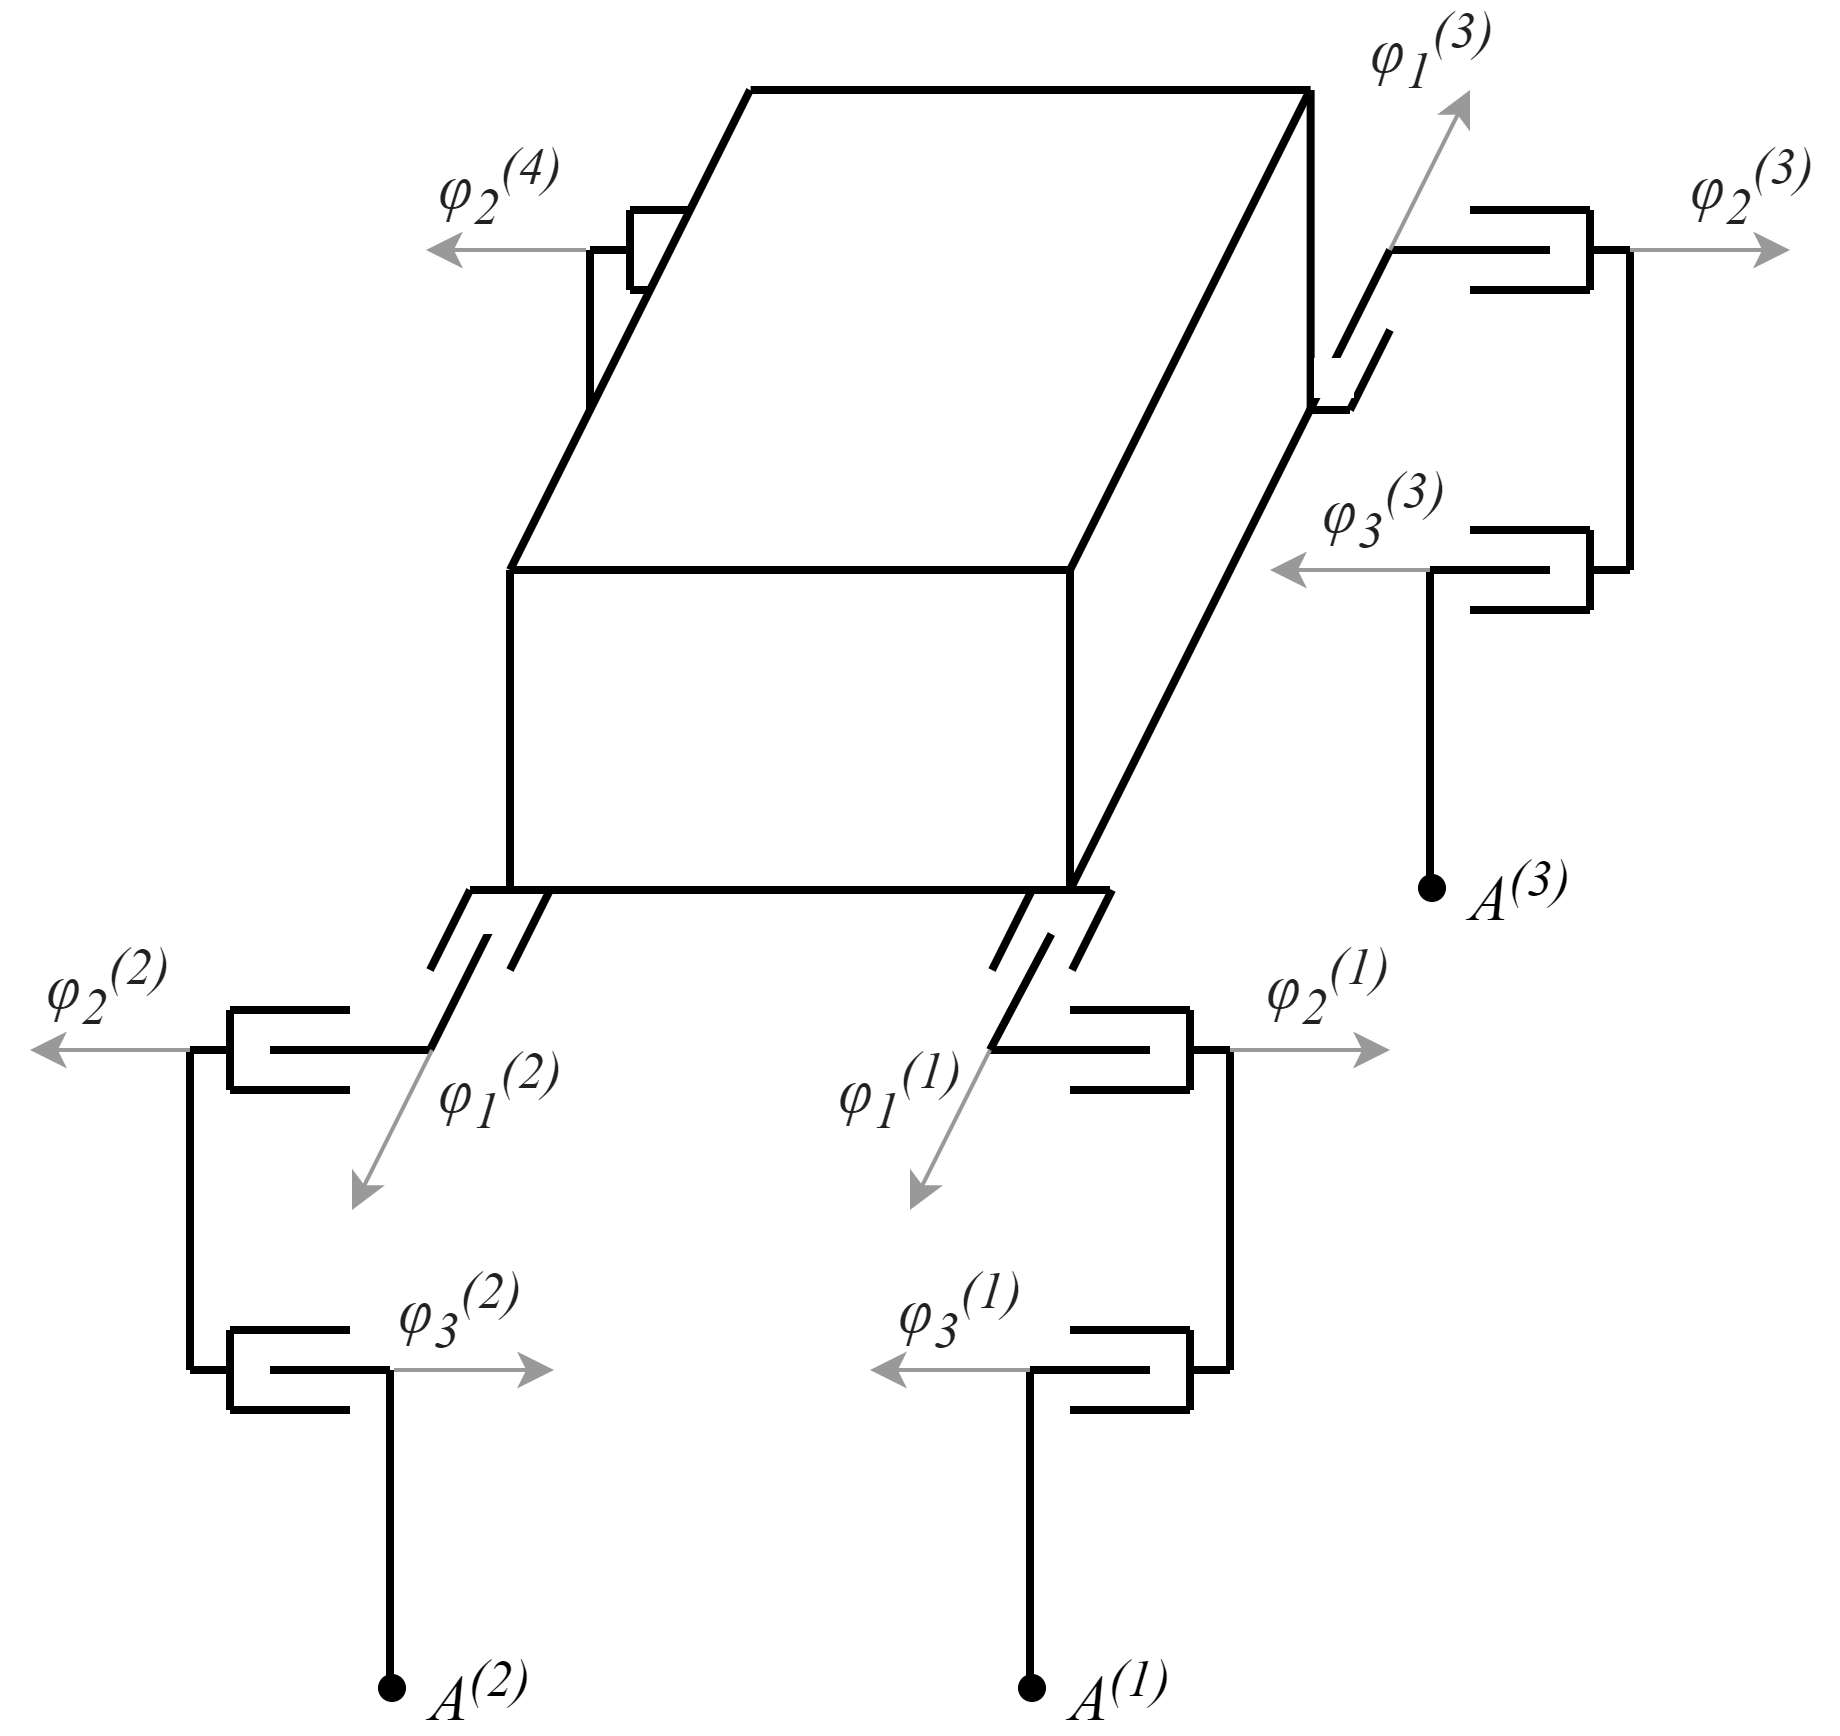
\includegraphics[scale=1.2]{chapter_legged_robots/figure1.png}
    \caption{Кинематика 4-х ногого робота. Нумерация ног произвольная}
    \label{fig:kin_scheme1}
\end{figure}

% \fixme ИЛЛЮСТРАЦИЯ

\subsection{Расчёт худшего статического случая}

Далее приведен расчёт, который был произведен уже после того, как чертежи прототипа были спроектированы, и такой структуре повествования требуется обоснование. Дело в том, что в конструкции прототипа изначально планировалось использовать сервоприводы. У большей части доступных на рынке сервоприводов одинаковые габариты, форма корпуса и даже расположение крепежных отверстий. Разница лишь в крутящих моментах, характеризующихся передаточным числом редуктора. Отсюда следует, что чертежи таких приводов ничем не отличаются друг от друга и это позволяет размещать их в сборочном чертеже робота до того как станет известна нагрузка на приводы. После того как становится известен точный набор комплектующих и их вес, а также длины конечностей, мы можем выбрать сервопривод, удовлетворяющий требуемому крутящему моменту.

Найдем максимальную статическую нагрузку на приводы конечностей рассмотрев наихудшую статическую конфигурацию робота. «Худшей» конфигурацией называется такая, при которой одному или нескольким приводам нужно приложить максимальный момент для поворота звена конечности в нужную сторону.

Конструкция ноги робота не позволяет разогнуть ее полностью. Поэтому можно привести длины звеньев конечности спроецированные на горизонтальную ось для того чтобы провести приблизительные расчеты:
\begin{align*}
    l_1 &\approx 131\: мм \\
    l_2 &\approx 134.5\: мм
\end{align*}

Худшим случаем является случай, при котором робот лежит на «животе» с выпрямленными конечностями. Чтобы подогнуть под себя конечность, нужно будет преодолеть момент $M_{худш}$ с учетом массы тела робота $m_T$. При этом максимальный крутящий момент потребуется приводу, находящемуся в первом узле, или можно сказать, управляющему первой степенью свободы.

\begin{figure}[ht]
    \centering
    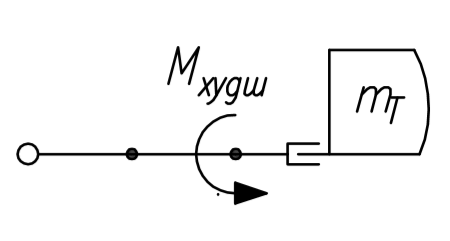
\includegraphics[scale=1]{kin2.png}
    \caption{Иллюстрация худшего статического случая}
\end{figure}
% на рисунке показать реакцию опоры и mg

При расчёте в первом приближении можно пренебречь трением и весами звеньев. Также можно учесть, что нагрузка, создаваемая массой тела робота будет распределена равномерно по всем четырем ногам. Это значит что на одну ногу будет приходится лишь $\frac{1}{4}m_T$ тела робота.

Самой тяжелой частью конструкции оказались каркас корпуса, в составе которого много аллюминиевых профилей, и аккумулятор. Самые легкие составляющие конструкции -- это электронные компоненты. Суммарно все комплектующие корпуса весят $3.2$ кг. 
% показать сколько килограмм набирается с комплектующих

При таком расчете можно считать что каждой ноге надо будет «поднять» около $ 0.8 $ кг веса. Тогда в худшем случае, приложенный момент вычисляется просто:
\begin{equation} \label{eq:statics1}
    M_{худш}= \frac 1 4 (l_{1}+l_{2}) m_T g, 
\end{equation}
\noindent здесь $l_1$ и $l_2$ - длины звеньев.

% перенести ближе к практической конструкторской части
При расчете по формуле \ref{eq:statics1} требуемый крутящий момент равен примерно $ 2.1  \: Н \cdot м$. После проведенного поиска среди доступных на рынке сервоприводов, был выбран сервопривод с крутящим моментом $ 2.5 \: Н \cdot м $. С таким сервоприводом максимально допустимый вес робота будет примерно равен $ 3.8 \: кг $.

Результат проектирования прототипа робота показан на рисунке \ref{fig:final_render}.

\begin{figure}[h]
    \centering
    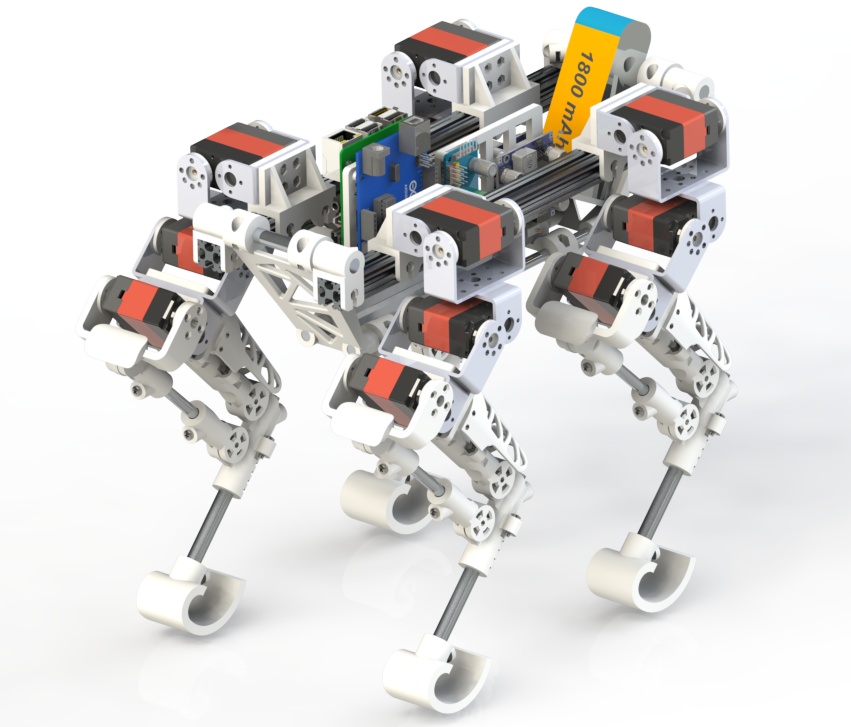
\includegraphics[width=0.85\textwidth]{chapter_mechanics_construction/figure20.png}
    \caption{Сборочный чертеж робота.}
    \label{fig:final_render}
\end{figure}

